\documentclass{article}

\usepackage{tikz}
\usetikzlibrary{shapes,arrows}
\usetikzlibrary{positioning}

\usepackage[scientific-notation=true, binary-units=true]{siunitx}
\sisetup{per-mode=fraction}%
\sisetup{scientific-notation=false}%
\usepackage[margin=2.5cm]{geometry}

\title{SYSC 4502 Assignment 3}
\date{March 24th, 2017}
\author{Jessica Morris \(100882290\)}

\tikzstyle{decision} = [diamond, draw, fill=white!20, 
    text width=4.5em, text badly centered, node distance=3cm, inner sep=0pt]
\tikzstyle{block} = [rectangle, draw, fill=white!20, 
    text width=5em, text centered, rounded corners, minimum height=4em]
\tikzstyle{line} = [draw, -latex']
\tikzstyle{cloud} = [draw, ellipse,fill=white!20, node distance=3cm,
    minimum height=2em]

\begin{document}

\maketitle

\begin{enumerate}

\item 
\begin{enumerate}
\item Block 1 arrives on time. Block 2 is delayed, as it arrives at a time $ t > t_1 + \Delta $. Blocks 4, 5 and 6 arrive on time. Block 3 arrives after $ t_1 > 2 \Delta $, so it is delayed. Block 7 arrives at time $ t > t_1 + 6 \Delta $, so it is delayed. So, four out of the seven blocks arrive on time.
\item If the client begins playout at $ t_1 + \Delta $, all blocks except for block 7 will have arrived on time to play. As determined in the previous question, blocks 2, 3, and 7 are delayed. Since the delay for blocks 2 and 3 is smaller than $\Delta$, while they are late, they still arrive on time for playback. Since block 7 has a delay greater than $\Delta$, it will be late.
\item At $t_1 + \Delta$ to $t_1 + 2\Delta$, block 2 is buffered, while block 1 is playing.
At $t_1 + 2\Delta$ to $t_1 + 3\Delta$, block 2 is played, while block 3 and block 4 are buffered.
At $t_1 + 3\Delta$ to $t_1 + 4\Delta$, block 3 is played, while block 4 and block 5 are buffered.
At $t_1 + 4\Delta$ to $t_1 + 5\Delta$, block 4 is played, while block 5 and block 6 are buffered.
At $t_1 + 5\Delta$ to $t_1 + 6\Delta$, block 5 is played, while block 6 is buffered.
At $t_1 + 6\Delta$ to $t_1 + 7\Delta$, block 6 is played.
At $t_1 + 7\Delta$ to $t_1 + 9\Delta$, nothing is played.
At $t_1 + 9\Delta$ to $t_1 + 10\Delta$, block 7 is played.

So, at most, 2 blocks are stored in the client buffer to await playout.
\item As per the previous question, an extra delay of $2\Delta$ at the client's end will cover the gap from the delay in receiving block 7; i.e., the client should start playing at $t_1 + 3\Delta$ to achieve a smooth playback.
\end{enumerate}

\item
\begin{enumerate}
\item For $ x < r $, the client will consume all of the playable bits in the application buffer after $ \frac{Q}{r-x} $ seconds. So, the playout period lasts $ \frac{Q}{r-x} $ seconds.

The number of bits to buffer for playing, $Q$, will refill at a rate of $x$ bits per second, and will take $Q/x$ seconds to fill. So, the freezing period is $Q/x$ seconds.

\item The application will consume the first $Q$ bits in the buffer at a rate of $x$. The remaining $B-Q$ bits in the buffer are consumed at a rate of $x-r$. So, the time it will take to fill the client's application buffer is given by:
$$ t_f = \frac{Q}{x} + \frac{B-Q}{x-r} $$

\end{enumerate}

\item The second leaky bucket generates tokens at rate $ r = p $, with bucket size $ b = 1 $. Placing this bucket in series with the first bucket means that the peak packet rate flowing from the first bucket will be controlled by the second bucket:

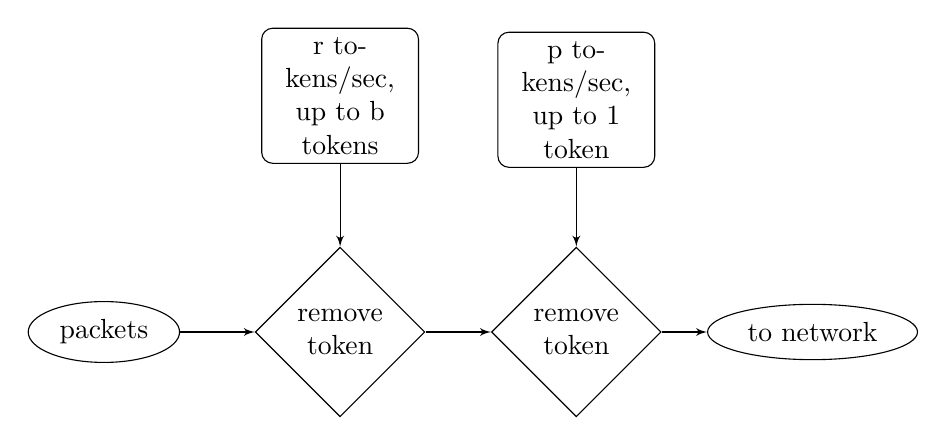
\begin{tikzpicture}[node distance = 2cm, auto]
    % Place nodes
    \node [block] (b1) {r tokens/sec, up to b tokens};
    \node [decision, below of=b1] (r1) {remove token};
    \node [cloud, left of=r1] (p1) {packets};
    \node [decision, right of=r1] (r2) {remove token};
    \node [block, above=1cm of r2] (b2) {p tokens/sec, up to 1 token};
    \node [cloud, right of=r2] (net) {to network};
    
    % Draw edges
    \path [line] (p1) -- (r1);
    \path [line] (b1) -- (r1);
    \path [line] (r1) -- (r2);
    \path [line] (b2) -- (r2);
    \path [line] (r2) -- (net);
\end{tikzpicture}

\item
\begin{enumerate}
\item For a FIFO queue service:

\begin{tabular}{|c|c|c|c|}
    \hline
    Packet & Arrive & Depart & Delay \\
    \hline
    1 & 0 & 1 & 0 \\ \hline
    2 & 0 & 2 & 1 \\ \hline
    3 & 1 & 3 & 1 \\ \hline
    4 & 1 & 4 & 2 \\ \hline
    5 & 3 & 6 & 2 \\ \hline
    6 & 2 & 5 & 2 \\ \hline
    7 & 3 & 7 & 3 \\ \hline
    8 & 5 & 8 & 2 \\ \hline
    9 & 5 & 9 & 3 \\ \hline
    10 & 7 & 10 & 2 \\ \hline
    11 & 8 & 11 & 2 \\ \hline
    12 & 8 & 12 & 3 \\ \hline
\end{tabular}

The average delay for the 12 packets is 1.9167.

\item For a priority queue service:

\begin{tabular}{|c|c|c|c|}
    \hline
    Packet & Arrive & Depart & Delay \\
    \hline
    1 & 0 & 1 & 0 \\ \hline
    2 & 0 & 3 & 2 \\ \hline
    3 & 1 & 2 & 0 \\ \hline
    4 & 1 & 7 & 5 \\ \hline
    5 & 3 & 4 & 0 \\ \hline
    6 & 2 & 8 & 5 \\ \hline
    7 & 3 & 5 & 1 \\ \hline
    8 & 5 & 10 & 4 \\ \hline
    9 & 5 & 6 & 0 \\ \hline
    10 & 7 & 11 & 3 \\ \hline
    11 & 8 & 9 & 0 \\ \hline
    12 & 8 & 12 & 3 \\ \hline
\end{tabular}

The average delay for the 12 packets is 1.9167.

\item For a round robin service:

\begin{tabular}{|c|c|c|c|}
    \hline
    Packet & Arrive & Depart & Delay \\
    \hline
    1 & 0 & 1 & 0 \\ \hline
    2 & 0 & 3 & 2 \\ \hline
    3 & 1 & 5 & 3 \\ \hline
    4 & 1 & 2 & 0 \\ \hline
    5 & 3 & 4 & 0 \\ \hline
    6 & 2 & 7 & 4 \\ \hline
    7 & 3 & 6 & 2 \\ \hline
    8 & 5 & 8 & 2 \\ \hline
    9 & 5 & 10 & 4 \\ \hline
    10 & 7 & 12 & 4 \\ \hline
    11 & 8 & 9 & 0 \\ \hline
    12 & 8 & 11 & 2 \\ \hline
\end{tabular}

The average delay for the 12 packets is 1.9167.

\item For a weighted fair queueing service:

\begin{tabular}{|c|c|c|c|}
    \hline
    Packet & Arrive & Depart & Delay \\
    \hline
    1 & 0 & 1 & 0 \\ \hline
    2 & 0 & 3 & 2 \\ \hline
    3 & 1 & 2 & 0 \\ \hline
    4 & 1 & 6 & 4 \\ \hline
    5 & 3 & 4 & 0 \\ \hline
    6 & 2 & 8 & 5 \\ \hline
    7 & 3 & 5 & 1 \\ \hline
    8 & 5 & 10 & 4 \\ \hline
    9 & 5 & 7 & 1 \\ \hline
    10 & 7 & 11 & 3 \\ \hline
    11 & 8 & 9 & 0 \\ \hline
    12 & 8 & 12 & 3 \\ \hline
\end{tabular}

The average delay for the 12 packets is 1.9167.

\item The average delay is the same for all four cases.
\end{enumerate}

\end{enumerate}
\end{document}
